\documentclass[informe.tex]{subfiles}
\begin{document}

\section{Gráfico (Alonso y Gabriela)}
Construya un gráfico que muestre cómo varían los tiempos de ejecución de sus cuatros soluciones en
nanosegundos, variando la cantidad $n$ de puntos entre las potencias de dos de $2^3=8$ a $2^9=512$.

\begin{figure}[h]
	\centering 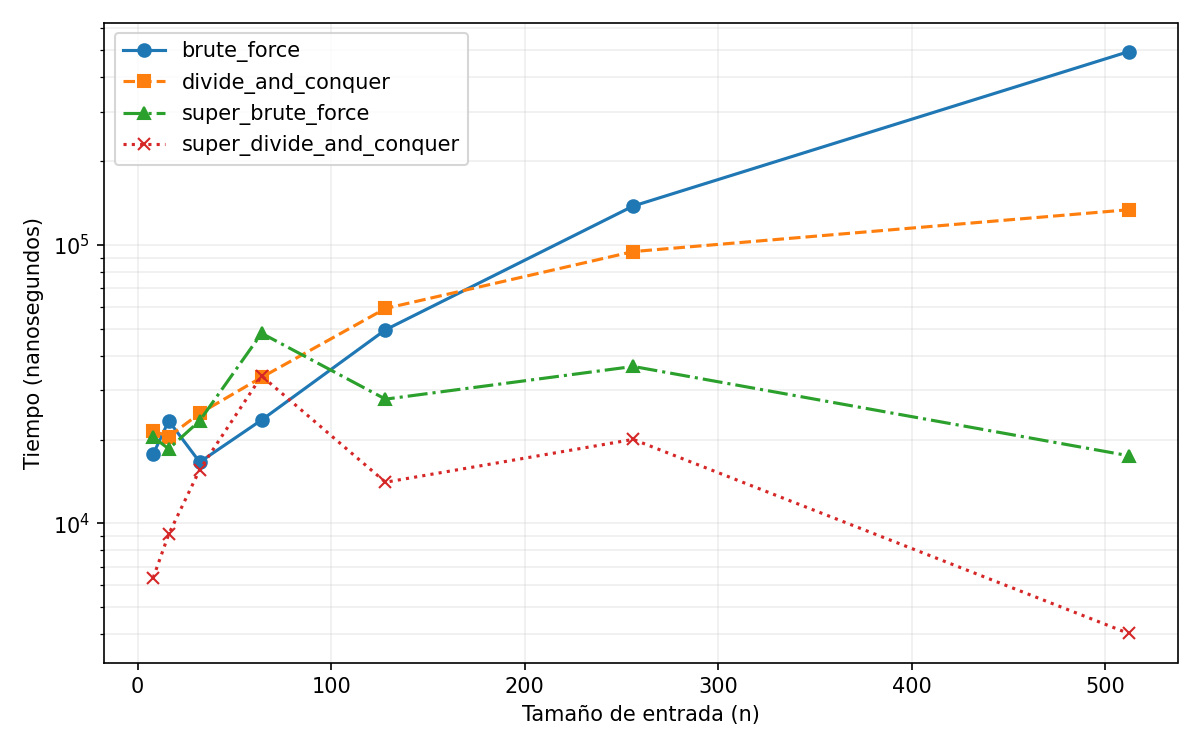
\includegraphics[width=0.8\textwidth]{img/plot_all.png}
\end{figure}

\end{document}
